\documentclass{article}
\usepackage[utf8]{inputenc}
\usepackage[sfdefault]{arimo}
\usepackage[T1]{fontenc}
\usepackage[margin=2cm]{geometry}

\usepackage{amsmath}
\usepackage{amsfonts}
\usepackage{mathrsfs} 
\usepackage{mathtools} 
\usepackage{amssymb}
\usepackage{hyperref}
\usepackage{float}
\usepackage{graphics}

\begin{document}\ \\
\ \\
\textbf{\underline{\Large{Electrical Engineering - Formula Sheet}}}\ \\
\section{BJT}
\begin{enumerate}
	\item KCL \[I_{E}=I_{C}+I_{B}\]
	\item CCCS \[\beta = \frac{I_{C}}{I_{B}} \quad \quad I_{C}=\alpha I_{E} \ (\alpha=\frac{\beta}{\beta +1})\]
	\item VCCS \[I_{C}=I_{S}e^{\frac{V_{BE}}{V_{T}}}\]\\In active mode: for npn BJT, $V_{BE}=0.7V$, for pnp BJT, $V_{EB}=0.7V$.  $V_{T}\approx 25.6mV$ under room temperature. \\\\A modified VCCS with the early voltage is  \[I_{C}=I_{S}e^{\frac{V_{BE}}{V_{T}}}(1+\frac{V_{CE}}{V_{A}})\]  $V_{CE,sat}\approx 0.2V$
	\item Output resistance \[r_{o}=\frac{V_{A}}{I_{C}}=\frac{\Delta v_{ce}}{\Delta i_{c}}\]
	\item Small signal transconductance \[g_{m}=\frac{I_{C}}{V_{T}}=\frac{\Delta i_{c}}{\Delta v_{be}}\quad \quad r_{e}=\frac{1}{g_{m}}\]
	\item Base input reisistance \[r_{\pi}=\frac{\beta}{g_{m}}=\frac{V_{T}}{I_{B}}\]
\begin{figure}[H]\centering
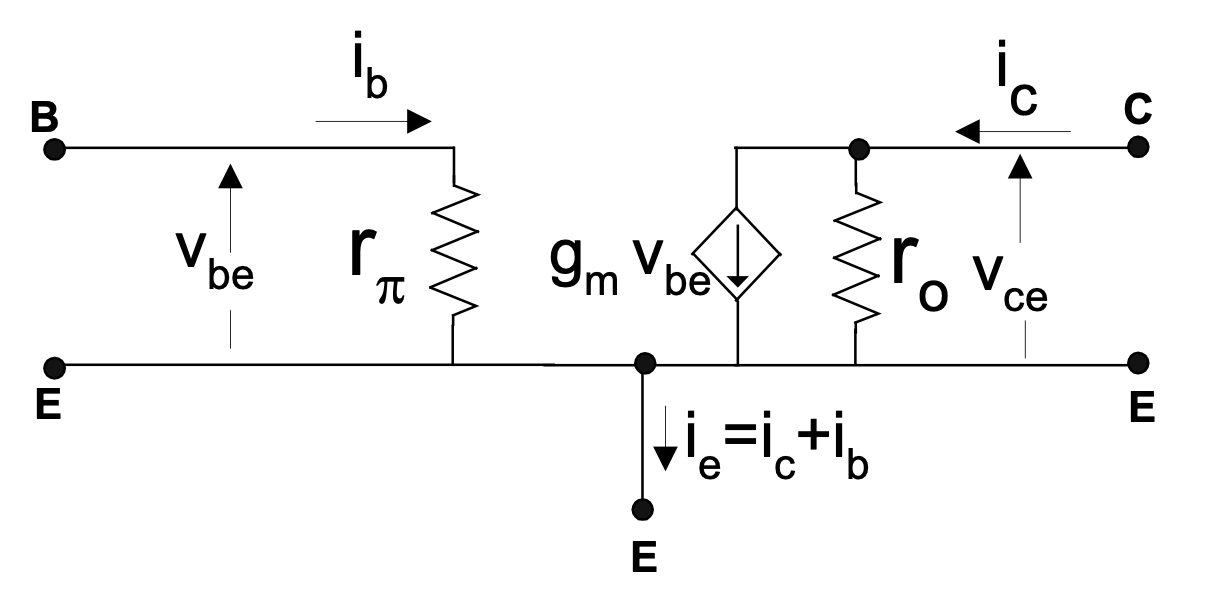
\includegraphics[width=.6\textwidth]{bjt_ss}
\caption{Small signal equivalent for BJT}
\end{figure}
\end{enumerate}

\section{MOSFET}
\begin{enumerate}
	\item $V_{GS}>V_{TH}$, $V_{DS}=0$, no induction current.
	\item Triode region $V_{GS}>V_{TH}$,  $V_{DS}<V_{GS}-V_{TH}$ \[i_{D} = \mu_{n}C_{ox}\frac{W}{L}(V_{GS}-V_{TH})V_{DS}\]
	\item Onset of saturation $V_{GS}>V_{TH}$,  $V_{DS}=V_{GS}-V_{TH}$ \[i_{D} = \frac{1}{2}\mu_{n}C_{ox}\frac{W}{L}(V_{GS}-V_{TH})^{2}\]
	\item Saturation $V_{GS}>V_{TH}$,  $V_{DS}>V_{GS}-V_{TH}$ \[i_{D} = \frac{1}{2}\mu_{n}C_{ox}\frac{W}{L}(V_{GS}-V_{TH})^{2}\] \\\ with the channel width modulation \[i_{D} =\frac{1}{2} \mu_{n}C_{ox}\frac{W}{L}(V_{GS}-V_{TH})^{2}(1+\lambda v_{DS})\] where $\lambda=\frac{1}{\lvert V_{A} \rvert}$
	\item Output resistance \[r_{o}=\frac{1}{\lambda i_{D}}=\frac{V_{A}}{i_{D}}\]
	\item Body effect equation \[V_{TH}=V_{TH,o}+\gamma[\sqrt{2\phi_{F}+V_{SB}}-\sqrt{2\phi_{F}}]\]
	\item Small signal transconductance \[g_{m}=\sqrt{2\mu_{n}C_{ox}}\sqrt{\frac{W}{L}}\sqrt{I_{D}}=\frac{2I_{D}}{V_{GS}-V_{TH}}\]
\end{enumerate}
\begin{figure}[H]\centering
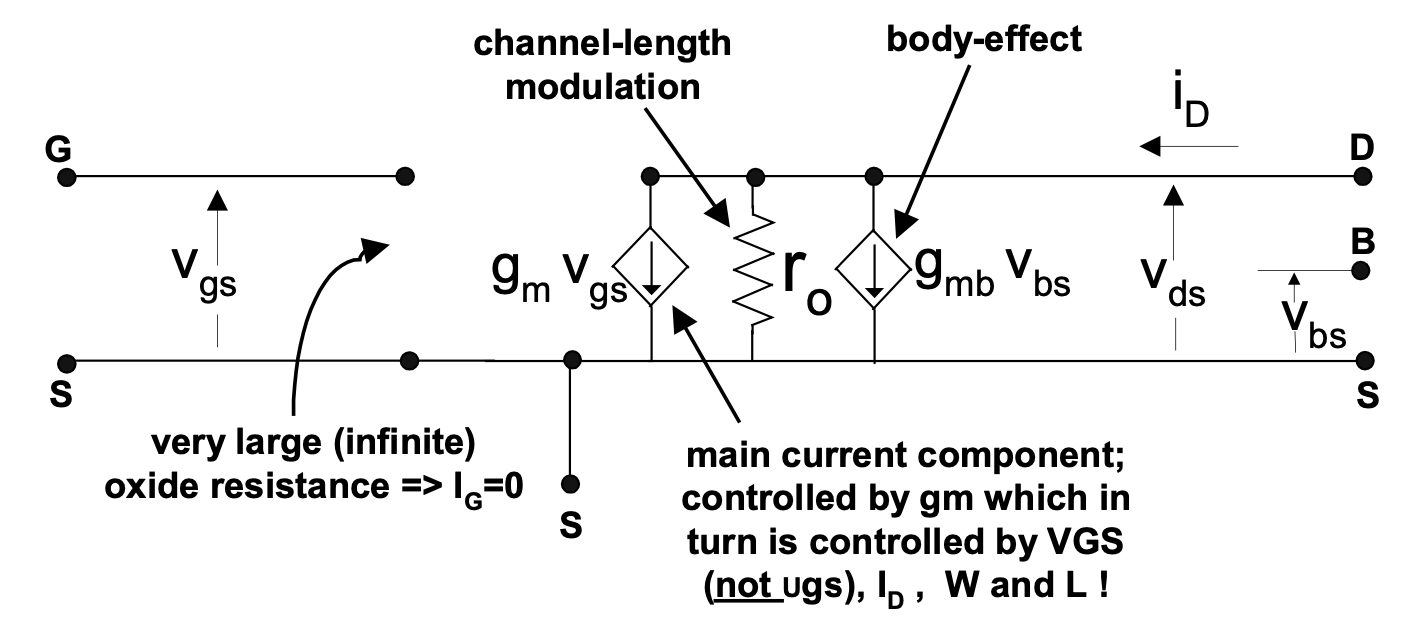
\includegraphics[width=.6\textwidth]{mos_ss}
\caption{Small signal equivalent for MOS}
\end{figure}

\section{Current Mirrors, Current and Voltage References}
\begin{enumerate}
	\item Simple current mirror \[\frac{I_{out}}{I_{in}}=\frac{1}{1+2/\beta} \quad \quad \frac{I_{out}}{I_{in^{'}}}=\frac{1+\frac{V_{CE,2}}{V_{A}}}{1+\frac{V_{CE,1}}{V_{A}}} \]
	\item $\beta$-compensated current mirror \[\frac{I_{out}}{I_{in}}=\frac{1}{1+2/\beta^{2}}\]
	\item MOS simple current mirror \[\frac{I_{out}}{I_{in}}=\frac{(\frac{W}{L})_{out}[1+\lambda v_{DS,out}]}{(\frac{W}{L})_{in}[1+\lambda v_{DS,in}]}\]
	\item $V_{BE}$-based ref \[I_{ref}=\frac{V_{EB}}{R}\]
	\item $V_{T}$-based ref \[I_{ref}=\frac{V_{T}}{R}\ln(\mu)\]
	\item $V_{BE}$ multiplier \[V_{out}=kV_{BE}\frac{(\frac{W}{L})_{5}}{(\frac{W}{L})_{2}}\]
	\item $V_{T}$ multiplier \[V_{out}=kV_{T}\ln(\mu)\]
	\item Bandgap reference \[\frac{\partial V_{EB}}{\partial T}=-2.2mV/ ^{\circ} C \quad \quad \frac{\partial V_{T}}{\partial T}=0.086mV/ ^{\circ} C\]
\[V_{out}=25.6V_{T}+V_{BE} \quad \quad V_{BG}=1.21-1.31V\]
\end{enumerate}

\section{Amplifiers}
\begin{table}[H] \centering \large
\begin{tabular}{|c|c|c|}
\hline
& Common Emitter & Common Emitter with Emitter Resistance\\ \hline
$A_{V}(\frac{V_{0}}{V_{i}})$ & $-\frac{R_{C}}{r_{e}}$ & $\approx -\frac{R_{C}}{R_{E}+r_{e}}$ \\  [1.3ex]\hline
$A_{VS}(\frac{V_{0}}{V_{S}})$ & $\frac{R_{b}\parallel R_{i}}{R_{S}+(R_{b}\parallel R_{i})}A_{V}$ & $\frac{R_{b}\parallel R_{i}}{R_{S}+(R_{b}\parallel R_{i})}A_{V}$\\ [1.3ex] \hline
%$A_{i}$ & $-\beta$ & $-\beta$ \\ [1.3ex] \hline
$R_{i}$ & $\approx \beta r_{e}$ & $\approx \beta (R_{E}+r_{e})$ \\ [1.3ex] \hline
$R_{out}$ & $R_{C}$ & $R_{C}$ \\ [1.3ex] \hline
\end{tabular}
\end{table}
\begin{figure}[H]\centering
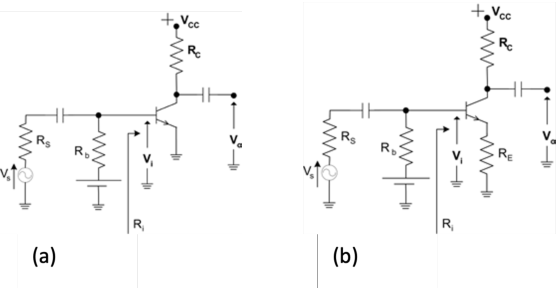
\includegraphics[width=.6\textwidth]{amp.pdf}
\caption{(a)Common emitter, (b)Common emitter with emitter resistance }
\end{figure}
\begin{itemize}
	\item DCLL \[I_{C}=-\frac{V_{CE}}{R_{C}}+\frac{V_{CC}}{R_{C}}\]
	\item ACLL \[i_{c}=-\frac{V_{CE}}{R_{C}\parallel R_{L}}+\frac{V_{CC}}{R_{C}\parallel R_{L}}-\frac{R_{C}}{R_{L}}I_{C}\]
	\item Optimal $Q$ \[I_{CQ^{*}}=\frac{1}{R_{C}\parallel R_{L}}\frac{R_{L}}{R_{C}+2R_{L}}V_{CC}\] \[V_{CEQ^{*}}=\frac{R_{L}}{R_{C}+2R_{L}}V_{CC}\]
	\item Intersection of ACLL and biasing line \[V_{CE}=V_{CC}-R_{C}I_{CQ}\]
	\item Emitter degenerated ACLL \[i_{c}=-\frac{V_{CE}}{R_{e}+(R_{C}\parallel R_{L})}+\frac{V_{CC}}{R_{e}+(R_{C}\parallel R_{L})}-\frac{R_{C}\parallel R_{L}}{R_{e}+(R_{C}\parallel R_{L})}\frac{R_{C}}{R_{L}}I_{C}\] \[I_{CQ}=\frac{1}{R_{e}+(R_{c}\parallel R_{L})}V_{CEQ} \quad \quad V_{CEQ}=\frac{R_{L}}{R_{C}+2R_{L}}V_{CC}\]
\begin{figure}[H]\centering
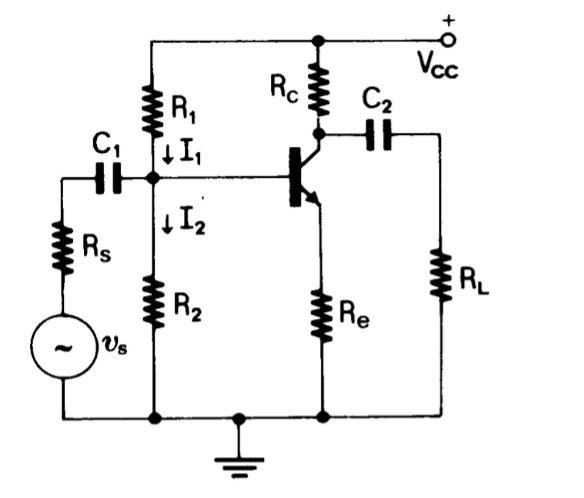
\includegraphics[width=.3\textwidth]{acll_re}
\end{figure}
	\item Emitter degenerated DCLL \[I_{C}=-\frac{V_{CE}}{R_{C}+R_{E}}+\frac{V_{CC}}{R_{C}+R_{E}}\]
\end{itemize}



\vspace*{\fill}
\framebox{\href{https://www.overleaf.com/read/tfgdmrfgypdc}{Scripted} by B Li \& P Xie. \ Last update: \today}
\end{document}
